\chapter{Implementation Details}
\label{ch:implementation}

This chapter elaborates on the algorithmic and procedural backbone of HiringGuru, focusing on backend processes and integration strategies that ensure operational integrity. Key workflows, system interactions, and validation mechanisms are discussed to demonstrate the robustness of the real-time mock interview platform.

%---------------------------------------------------------------------
\section{Core Algorithmic Workflows}
HiringGuru relies on several critical algorithms and processes to deliver AI-driven interview feedback:

\subsection{Authentication Protocol}
The authentication mechanism uses Firebase Authentication, leveraging secure token-based access with JSON Web Tokens (JWT) for session management (Figure~\ref{fig:architecture}). User credentials are hashed using bcrypt, ensuring no plaintext storage. The workflow verifies user identity and authorizes access to interview sessions.

\subsection{Real-Time Analysis Pipeline}
The pipeline processes webcam input for posture, facial expression, and eye contact analysis:
\begin{itemize}
    \item \textbf{Step 1}: Webcam frames are preprocessed using OpenCV (CV2) for grayscaling and noise reduction.
    \item \textbf{Step 2}: MobileNetV2 and MediaPipe analyze posture, achieving 90\% accuracy, while Haarcascade and Dlib handle facial expression and eye contact detection, respectively.
    \item \textbf{Step 3}: Analysis results are aggregated and stored in Firebase for real-time feedback generation.
\end{itemize}

\subsection{Question Generation Workflow}
The OpenAI API generates contextually relevant interview questions based on user profiles and job roles. Questions are cached in memory to minimize API calls, ensuring low-latency delivery during interview sessions.

%---------------------------------------------------------------------
\section{System Interaction Model}
Figure~\ref{fig:sequential-model} illustrates the sequential processing of user interactions, from authentication to feedback delivery. The UML Use Case Diagram below details actor-use case relationships, highlighting the interactions between users and the system.

\begin{figure}[h]
  \centering
  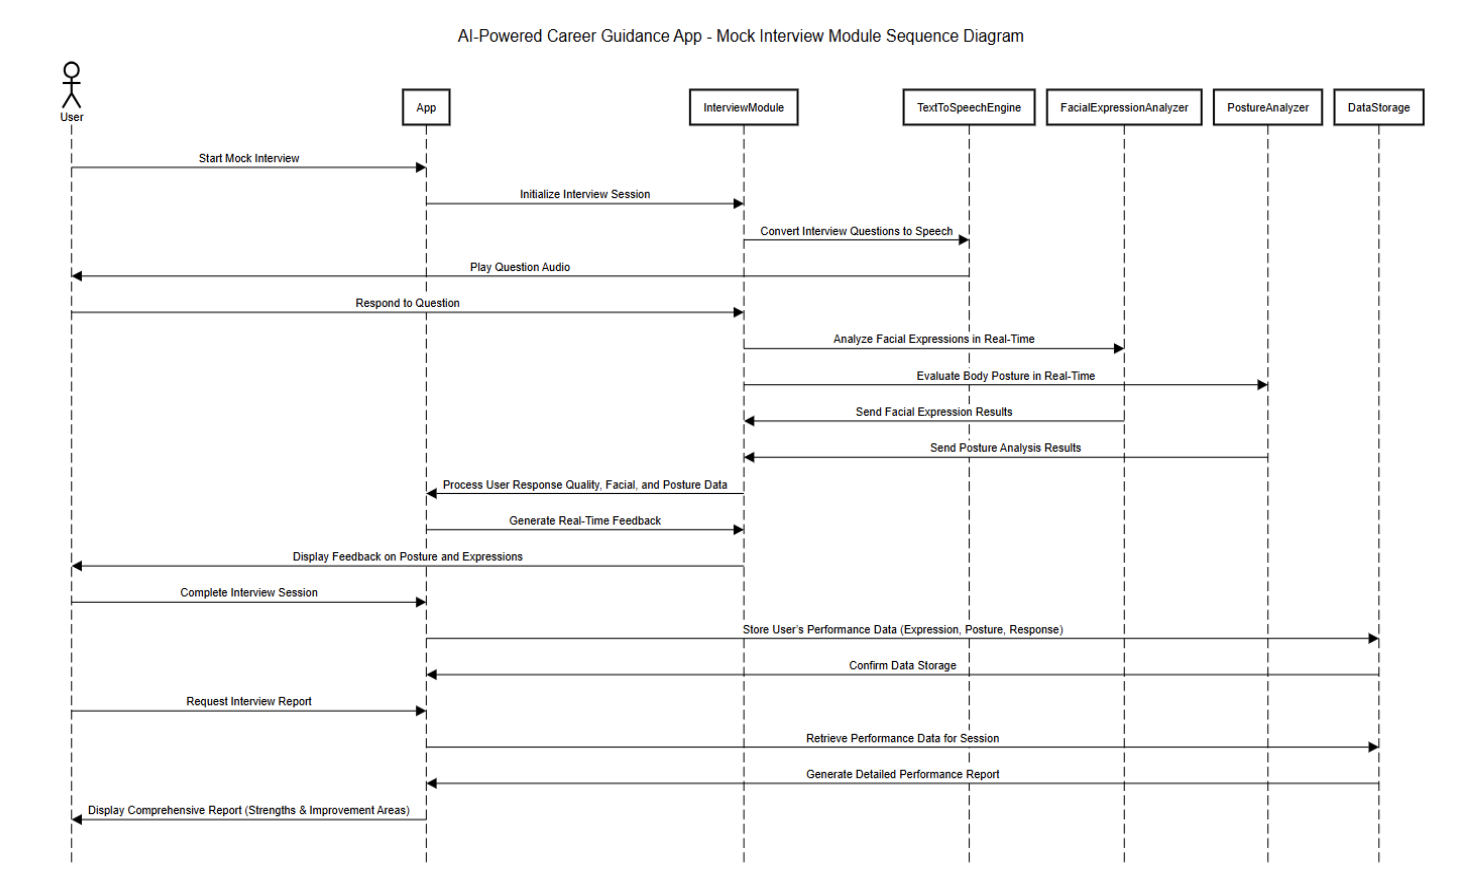
\includegraphics[width=0.9\textwidth]{sections/diagrams/SequentialModel.png}
  \caption{Sequential processing model for user requests}
  \label{fig:sequential-model}
\end{figure}

% UML Use Case Diagram for HiringGuru
\begin{figure}[h]
\centering
\begin{tikzpicture}
% System Boundary
\begin{umlsystem}[x=4, fill=blue!5]{HiringGuru}
  \umlusecase[name=startInterview, x=2, y=0]{Start Interview}
  \umlusecase[name=analyzePosture, x=2, y=-2]{Analyze Posture}
  \umlusecase[name=generateFeedback, x=2, y=-4]{Generate Feedback}
  \umlusecase[name=manageQuestions, x=6, y=-2]{Manage Questions}
\end{umlsystem}

% Actors
\umlactor[x=-2, y=0]{User}
\umlactor[x=12, y=-2]{Admin}

% Relationships
\umlassoc{User}{startInterview}
\umlassoc{Admin}{manageQuestions}
\umlinclude{startInterview}{analyzePosture}
\umlVHextend{generateFeedback}{startInterview}

% Note
\umlnote[x=6, y=-6]{Note}{"Start Interview" includes posture analysis and may extend to feedback generation.}
\end{tikzpicture}
\caption{UML Use Case Diagram for HiringGuru}
\label{fig:uml-usecase}
\end{figure}

%---------------------------------------------------------------------
\section{Architecture Integration}
As shown in Figure~\ref{fig:architecture}, HiringGuru adopts a layered architecture to ensure modularity and scalability:

\begin{figure}[h]
  \centering
  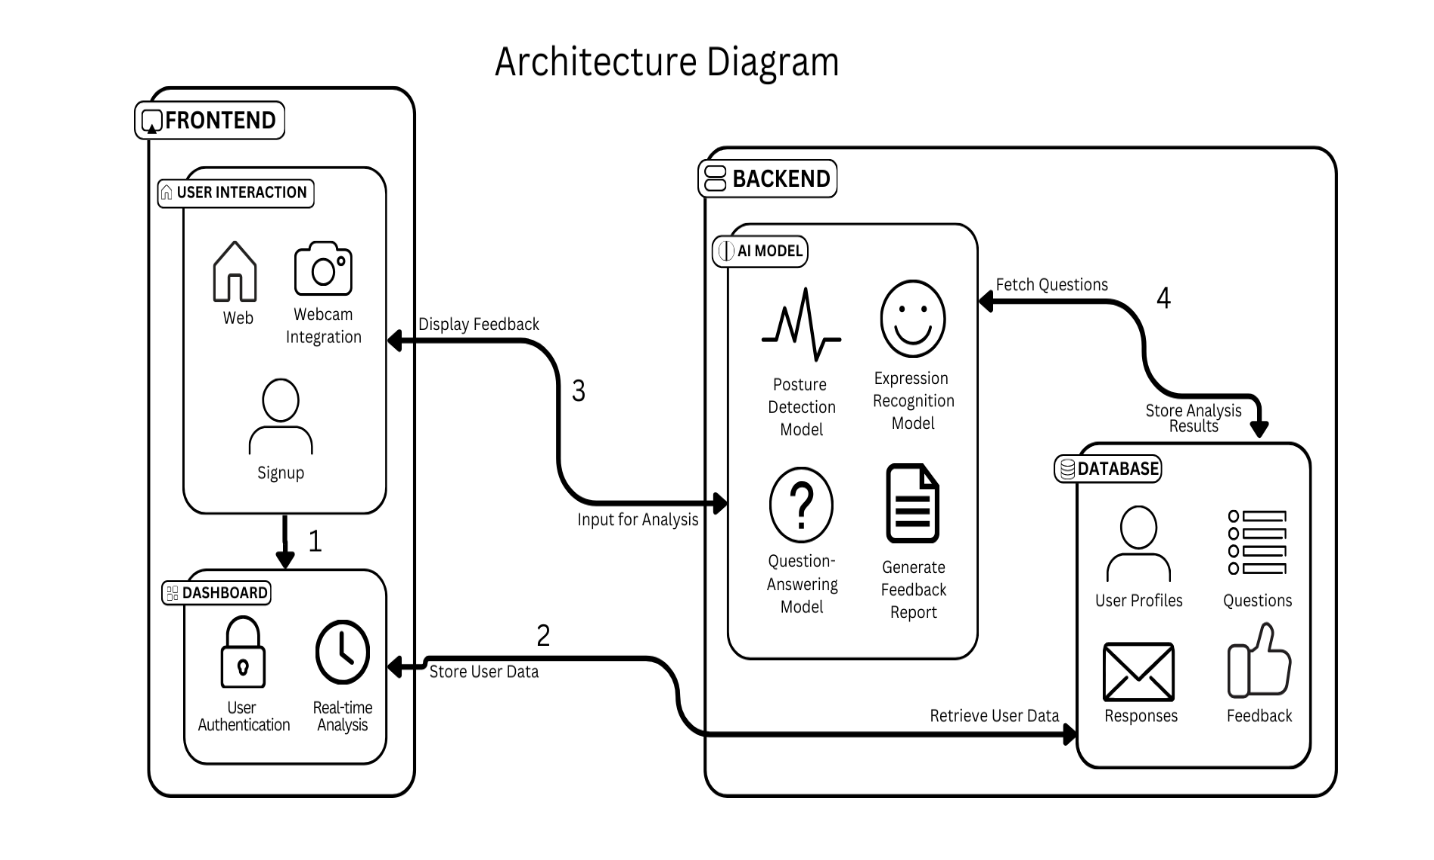
\includegraphics[width=0.85\textwidth]{sections/diagrams/ArchitectureDiagram.png}
  \caption{High-level system architecture}
  \label{fig:architecture}
\end{figure}

\begin{itemize}
    \item \textbf{Frontend}: Built with Next.js and TailwindCSS, providing a responsive user interface for interview sessions.
    \item \textbf{Backend}: Node.js handles business logic, coordinating between AI analysis modules and Firebase.
    \item \textbf{AI Analysis}: TensorFlow, MediaPipe, Haarcascade, and Dlib process webcam input for real-time feedback.
    \item \textbf{Data Storage}: Firebase provides real-time database and authentication services, with optimized queries for analysis results.
\end{itemize}

%---------------------------------------------------------------------
\section{Validation \& Testing}
HiringGuru’s implementation was rigorously validated to ensure reliability and performance:
\begin{itemize}
    \item \textbf{Unit Testing}: Validated individual components, such as MobileNetV2 posture detection and OpenAI API integration, using Jest and PyTest.
    \item \textbf{Integration Testing}: Ensured seamless interaction between frontend, backend, and AI modules, testing scenarios like varying lighting conditions.
    \item \textbf{Performance Testing}: Simulated 1,000 concurrent users to verify system scalability, achieving sub-2-second response times.
    \item \textbf{Security Testing}: Conducted penetration tests to address vulnerabilities, ensuring compliance with secure coding practices.
\end{itemize}

%---------------------------------------------------------------------
\section{Summary}
HiringGuru’s implementation achieves its design objectives through:
\begin{itemize}
    \item Optimized algorithms for real-time posture, facial expression, and eye contact analysis.
    \item A modular architecture enabling seamless integration of AI and web components.
    \item Comprehensive testing to ensure reliability, scalability, and security.
\end{itemize}